% =====================================================================
% Draft section — the payoff section of the epistasis paper.
% Argument: the preceding sections rank discovery methods by retained
% interaction structure. This section shows what that structure contains,
% and therefore what an additive circuit discards.
%
% Status: first draft, unreviewed. Compiles clean standalone.
% Requires: booktabs, amsmath, amssymb, natbib (\citet/\citep).
% Bib entries still needed: wang2022ioi, benzer1955.
% \ref{tab:energy} points at the existing energy-fraction table — check
% the label matches before wiring this in.
% =====================================================================

\section{What the interaction structure contains}
\label{sec:what-epistasis-contains}

The preceding sections rank discovery methods by the interaction structure they retain.
That ranking earns its place only if the retained structure carries mechanism, so this
section asks what is inside the order-2 spectrum of a circuit whose mechanism is already
documented. Reading the canonical indirect object identification circuit of
\citet{wang2022ioi} against its own taxonomy recovers a dependency between two of its head
classes that the published account records as unexplained.

\subsection{Double ablation decides whether two components are one unit}

Genetics has decided whether two mutations belong to one unit or two since the 1950s, using
a test that requires no knowledge of what the unit is made of. Two recessive mutations are
placed in \emph{trans}, and the phenotype of the double heterozygote decides one locus or
two \citep{benzer1955}. The reading is a sign convention on the interaction between the two
perturbations:

\begin{center}
\begin{tabular}{lll}
\toprule
interaction & reading & verdict \\
\midrule
sub-additive (masking) & one pathway; the second hit has nothing left to break & same unit \\
additive & independent pathways & different units \\
super-additive (synergy) & parallel pathways, each covering for the other & different units \\
\bottomrule
\end{tabular}
\end{center}

An exhaustive coalition sweep supplies exactly this data for every head pair at once. For a
circuit of $n$ heads, the $2^n$ coalition values determine every order-2 Walsh coefficient
$w_{ij}$ exactly, with no regularization and no held-out set. Taking $M_{ij} = -w_{ij}$
under the convention above yields a signed masking matrix over all $\binom{n}{2}$ pairs.
Magnitude alone is uninterpretable here, since masking and synergy are both large
$|w_{ij}|$; the sign carries the verdict.

Interpretability assigns head roles from what a head appears to do. Applying the
complementation test to those roles asks whether the names track a functional criterion.

\subsection{The taxonomy separates induction and name-mover heads, and merges two others}

Hierarchical clustering on $M$ for the 15-head IOI circuit, with cluster count selected by
silhouette, recovers induction heads (L5H5, L6H9) and name-mover heads (L9H9, L10H0) as
exact units. Adjusted Rand Index against the published labels is $+0.571$ as a point
estimate, with a bootstrap-over-prompts 95\% interval of $[+0.125, +0.571]$. The taxonomy
therefore tracks interaction structure, by an amount the resampling leaves uncertain.

One boundary fails, and it fails stably. S-inhibition heads and negative name movers occupy
a single cluster in \textbf{1000 of 1000} bootstrap resamples, while the global partition
wobbles across the same draws. The merge holds in every robustness condition we ran: mean
ablation as well as zero, circuits from EAP-IG and from order-1 Walsh discovery as well as
the order-2 circuit, and complete and Ward linkage as well as average. Under a larger set of
role labels the bootstrap merge rate falls to $81$--$86\%$ on the zero-ablation conditions
and remains at $100\%$ on the others, so the pair separates occasionally once the clustering
has more classes available to it.

Depth does not explain this. Roles in IOI are layer-stratified, so a clustering that
recovered depth would score well against roles by accident. The derived partition matches
role at ARI $0.571$, raw layer at $0.053$, and layer band at $0.217$, while role itself
matches layer band at $0.526$. The clustering tracks role an order of magnitude better than
depth.

\subsection{The merge is asymmetric, and the asymmetry is the result}

Figure 2 of \citet{wang2022ioi} places name movers, negative name movers, and backup name
movers inside one group, with S-inhibition writing the queries of all three. On that
topology, removing S-inhibition disables what the group does, and a merge between
S-inhibition and any member follows.

The data merge one member and separate the other:

\begin{center}
\begin{tabular}{lc}
\toprule
class pair & merged in \\
\midrule
S-inhibition $\sim$ negative name mover & 4 / 4 conditions \\
S-inhibition $\sim$ name mover & 0 / 2 conditions \\
name mover $\sim$ negative name mover & 0 / 2 conditions \\
\bottomrule
\end{tabular}
\end{center}

\citet{wang2022ioi} state the only difference between the two classes: the negative heads
``share all the same properties as Name Mover Heads except they (1) write in the opposite
direction of names they attend to and (2) have a large negative copy score.'' Same query
source, same key and value input, same output edge, opposite OV sign. A topological account
of the merge predicts that S-inhibition masks both classes, and the circuit diagram has no
element that would distinguish them.

\subsection{The negative heads invert rather than diminish}

The OV sign difference predicts the asymmetry. Negative name movers write the negation of
whatever they attend to. With S-inhibition intact they attend to the indirect object and
write $-\mathrm{IO}$, which lowers the logit difference. Removing S-inhibition redirects
their attention to the subject, so they write $-\mathrm{S}$, which \emph{raises} the logit
difference $\mathrm{IO} - \mathrm{S}$. Their contribution inverts. Name movers copy
positively, so losing S-inhibition degrades them toward zero without changing their sign.

The exhaustive lattice tests this directly. Restricting to coalitions in which all
S-inhibition heads are retained, and separately to those in which all are removed, the
marginal contribution $\mathbb{E}_S[v(S \cup \{i\}) - v(S)]$ is exact in each condition:

\begin{center}
\begin{tabular}{llrrr}
\toprule
class & head & S-inh.\ retained & S-inh.\ removed & sign flips \\
\midrule
negative name mover & L10H7  & $-0.130$ & $+0.137$ & 1000 / 1000 \\
negative name mover & L11H10 & $-0.057$ & $+0.180$ & 1000 / 1000 \\
name mover          & L9H9   & $+0.129$ & $-0.012$ & 878 / 1000 \\
name mover          & L10H0  & $+0.149$ & $+0.009$ & 318 / 1000 \\
\bottomrule
\end{tabular}
\end{center}

Figure~\ref{fig:conditional-marginal} visualizes the pattern. Both negative heads invert in
every bootstrap draw, moving from clearly harmful to clearly helpful. The name movers decay toward zero: L10H0 keeps its sign, and L9H9 crosses zero at a
magnitude of $0.012$, which is indistinguishable from no contribution at all. Sign reversal and neutralization are distinct outcomes. They produce the two
interaction signs the clustering found: S-inhibition with negative name movers
gives $-0.267$ (masking, one unit), while S-inhibition with name movers gives
$+0.141$ (synergy, two units).

\begin{figure}[t]
\centering
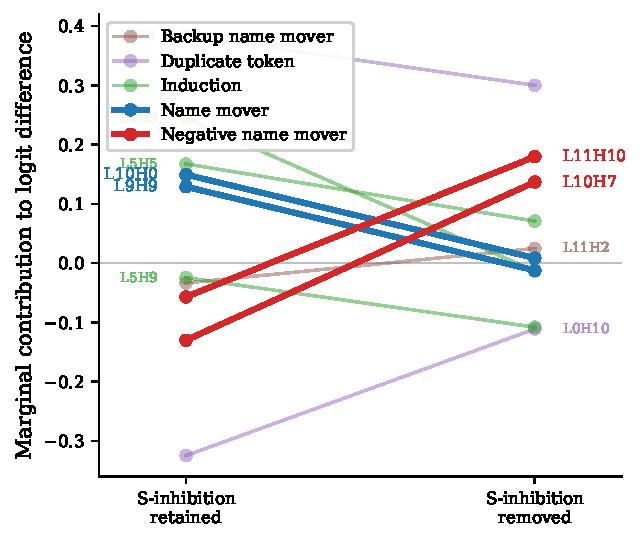
\includegraphics[width=0.65\textwidth]{figures/conditional_marginal.pdf}
\caption{Marginal contribution of each head to logit difference,
conditioned on whether S-inhibition heads are retained (left) or removed
(right). The two negative name movers (red) cross zero, inverting from
harmful to helpful. Name movers (blue) decay toward zero without
inverting. Other head classes show moderate attenuation. Bootstrap sign-flip
rates: both negative name movers flip in 1000/1000 draws.}
\label{fig:conditional-marginal}
\end{figure}

\citet{wang2022ioi} observed a fragment of this effect under a different conditioning set.
After knocking out name movers, they report that ``the Negative Name Mover Heads have a less
negative effect on logit difference, and 10.7 even has a positive effect on the logit
difference after the knockout,'' and conclude that ``[b]oth the reason and the mechanism of
this compensation effect are still unclear.'' Path patching measures one edge against a
fixed background, which makes a dependency of this kind visible only where the background
happens to expose it. The interaction decomposition holds the whole lattice, so the
dependency appears for both heads, with a magnitude and a stability attached.

\subsection{What an additive circuit discards}

This dependency lives entirely in order-2. A circuit summarized by its order-1 coefficients
retains that negative name movers lower the logit difference on average, and loses that the
sign of their contribution is set by an upstream class. The EAP-IG circuit
carries $90.4\%$ of its energy at order 1 against the canonical circuit's $78.6\%$
(Table~\ref{tab:energy}), and that gap is the room in which effects like the sign inversion sit.

\begin{table}[h]
\centering
\begin{tabular}{lccc}
\toprule
Circuit & Order 1 (\%) & Order 2 (\%) & Order 3{+} (\%) \\
\midrule
EAP-ranked           & 90.4 & 9.0  & 0.6 \\
Canonical (Wang)     & 78.6 & 18.4 & 3.0 \\
Walsh-ranked         & 80.9 & 16.8 & 2.3 \\
Epistasis-ranked     & 78.4 & 18.6 & 3.0 \\
Random               & 97.9 & 2.1  & 0.0 \\
\bottomrule
\end{tabular}
\caption{Fraction of nonconstant Walsh energy at each interaction order
for five 15-head IOI circuits under mean ablation. The EAP-ranked circuit
concentrates energy at order 1; circuits selected for functional relevance
(canonical, Walsh, epistasis) retain 17--19\% at order 2.}
\label{tab:energy}
\end{table}

The consequence for practice is narrow and concrete. A head's measured contribution is a
property of the head together with the background it was measured against, and reporting it
as a property of the head alone is safe only when the order-2 terms coupling it to the rest
of the circuit are small. Those terms are measurable, so the assumption is checkable rather
than assumed.

% ---------------------------------------------------------------------
% NOTES FOR REVISION
%
% 1. Figure to make: conditional marginal contribution for all labelled
%    heads, S-inh retained vs removed, as a slope chart. The two negative
%    heads cross zero in opposite direction to everything else — that is
%    the whole result in one image. Data: results/v13_conditional_marginal.json
%
% 2. Scope sentence still owed somewhere in this section or in limitations:
%    one model (GPT-2 small), one task (IOI), merge rests on five heads,
%    sign-flip result on two. Whether sign inversion generalizes to other
%    inhibitory pairings is untested.
%
% 3. Provenance sentence owed in methods: the complementation analysis was
%    preregistered (prereg_v13, sha 1f915bbc, amended e258d592); the
%    conditional-marginal test in 4.4 was derived from the pairwise result
%    and is a follow-up rather than a registered prediction. One sentence,
%    methods only.
%
% 4. The ARI numbers here are from the registered 10-label analysis. A later
%    run with an expanded 18-label dictionary gives lower ARIs (0.106-0.290,
%    one negative). Do not mix the two sets in one table. The merge holds
%    under both; only the merge should be quoted across label sets.
%
% 5. Table \ref{tab:energy} is the existing energy-fraction table from the
%    results section; check the label matches before compiling.
% ---------------------------------------------------------------------
